Bei der Erforschung des hei{\ss}en und dichten Mediums beziehungsweise der Suche nach dem QGP spielt das Phasendiagramm stark wechselwirkender Materie eine wichtige Rolle.
\begin{figure}[tbp]
\centering
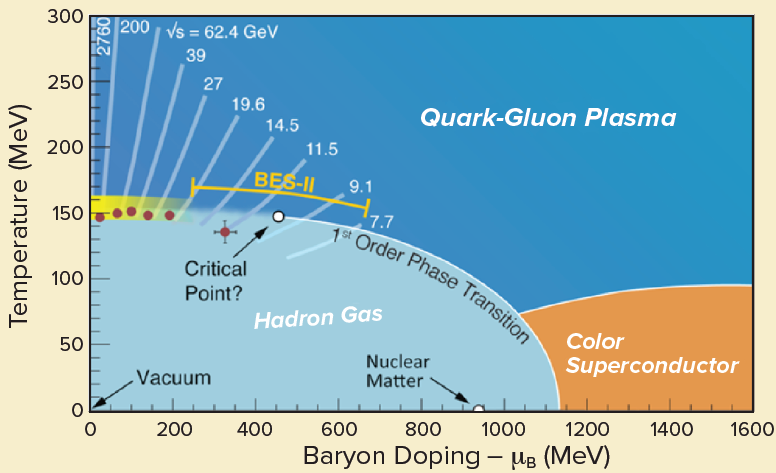
\includegraphics[width=.7\linewidth]{QGPPhaseDiagram.png}
\caption{Phasendiagramm stark wechselwirkender Materie in Abh\"angigkeit der Baryonendichte $\mu_{\text{B}}$ und der Temperatur $T$.
[https://arxiv.org/abs/1609.03104]}
\label{fig:QGPPhase}
\end{figure}
Abbildung \ref{fig:QGPPhase} skizziert ein Phasendiagramm stark wechselwirkender Materie in Abh\"angigkeit der Baryonendichte $\mu_{\text{B}}$ und der Temperatur $T$.
Bei geringer Baryonendichte und niedriger Temperatur, wie etwa Raumtemperatur, sind alle Quarks und Gluonen in Hadronen gebunden.
Erh\"oht man die Temperatur, oder beide Gr\"o{\ss}en, stark wird ein \"Ubergang in das QGP erwartet, in welchem sich die Quarks und Gluonen quasi frei bewegen k\"onnen.
Au{\ss}erdem muss die Energiedichte gro{\ss} genug sein um ein QGP erzeugen zu k\"onnen, weshalb davon ausgegangen wird, dass sich dieses nur bei Kernkollisionen ausbilden kann.
Proton-Proton-Kollisionen werden als Referenzmessungen benutzt.

In der Abbildung sind zus\"atzlich verschiedene Schwerpunktsenergieen $\sqrt{s}$ eingezeichnet.
Die Schwerpunktsenergie eines Kollisionsexperiments gibt an, wie viel Energie dem System bei der Kollision zur Verf\"ugung steht.
Entsprechend h\"angt $\sqrt{s}$ von der Energie der kollidierende Teilchen oder Kerne ab.
F\"ur Kollisionsexperimente zweier identischer Teilchen oder Kerne mit gleicher Energie $E$ gilt:
\begin{align}
\sqrt{s} = 2E \label{eq:sqrts}
\end{align}
Unterschiedliche $\sqrt{s}$ liefern also Daten aus unterschiedlichen Bereichen des Phasendiagramms.
Um die Bereiche des Phasendiagramms innerhalb des QGP und dem \"Ubergang zwischen quasi freien zu gebundenen Quarks und Gluonen untersuchen zu k\"onnen, werden also Kollisionen mit ausreichenden Schwerpunktsenergieen ben\"otigt.

Um die ben\"otigten Scherpunktsenergieen erreichen zu k\"onnen, m\"ussen die Teilchen beziehungsweise Kerne auf fast Lichtgeschwindigkeit beschleunigt werden.
Die Beschleunigung geschieht in Beschleunigerringen, wo die Teilchen oder Kerne durch Dipolmagnete auf einer Kreisbahn gehalten und durch elektrische Felder beschleunigt werden.
Der LHC, der weltweit gr\"o{\ss}te Beschleunigerring, geh\"ohrt zu CERN und erreicht aktuell Schwerpunktsenergieen bis $\sqrt{s} = 13 TeV$.
Im LHC Ring befinden sich vier Punkte an denen Kollisionen stattfinden.
An diesen vier befinden sich umfangreiche Detektorkomplexe, wie etwa der ALICE Detektor.
Im folgenden Abschnitt wird das ALICE Experiment genauer beschrieben.